\chapter{Questioning the robustness of synaptic
plasticity rules to neuromodulation, cellular and
network perturbations}

\begin{shaded}
BLABLABLA\\
BLABLABLA\\
~\\
Presented at the Annual Meeting of the Belgian Society for Neuroscience in 2022 (oral presentation - Brussels)
\end{shaded}

% ---------------------------------------------
% ---------------------------------------------
%
%       SMALL COMPUTATIONAL EXPERIMENTS 
%   TO SHOW INCOMPATIBILITY BETWEEN VAR & SP 
%
% ---------------------------------------------
% ---------------------------------------------

\section{Introduction}
- switches in neuronal activity\\
- neuromodulation\\
- Figure \ref{fig:intro}\\
- ...\\

\begin{figure}[h!]
    \centering
    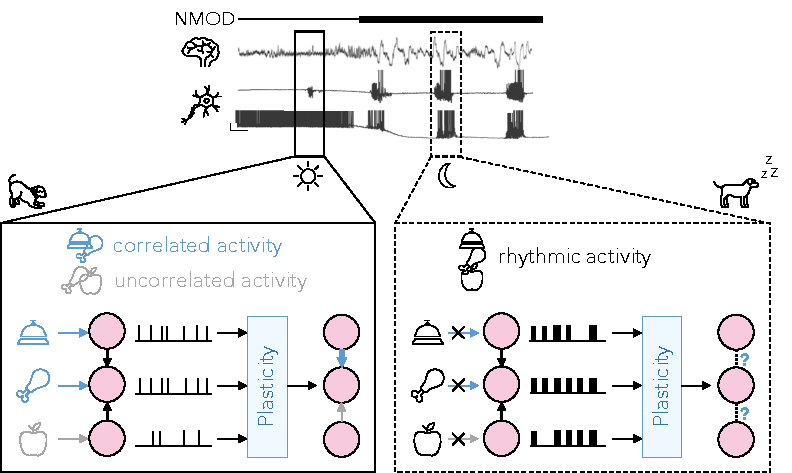
\includegraphics{fig/Review/fig_intro.pdf}
    \caption{\textbf{The impact of switches in brain states, neuronal activity onto synaptic plasticity remains unclear.} (Top) Switches in brain states (recorded by EEG signal) reflecting switches in neuronal firing activity are orchestrated by neuromodulators  (adapted from \cite{zagha_neural_2014}). (Bottom-left) During tonic firing associated to an active state, correlated neurons (bell-chicken) increase their synaptic weights while uncorrelated neurons (chicken-appel) decrease the weights. (Bottom-right) During synchronized bursting associated to a quiet state, external inputs are disconnected, neurons are bursting; synaptic change is not yet elucidated.  }
    \label{fig:intro}
\end{figure}



%%%%%%%%%%%%%%%%%%
vestiges de la review: \\
\begin{comment}
\textcolor{orange}{Je pense qu'on peut enlever ce paragraphe: c'etait pour indiquer comme c'etait compliqué de fitter le calcium car on n'a pas accès à des données clairement quantifiées}\\
\color{gray}
It is also important to not that fitting a calcium-dependent synaptic rule is challenging. Indeed,  recording internal calcium measure is complex. It requires fluorescent data from experiments. In addition to build a model based biological calcium amplitude and time-evolution,  lot of plasticity induction protocols exist such as:  \citep{yang_selective_1999, sjostrom_rate_2001, sjostrom_cooperative_2006, wittenberg_malleability_2006, nevian_spine_2006, letzkus_learning_2006, wang_coactivation_2005, paille_gabaergic_2013, fino_distinct_2010, frey_synaptic_1997, dudek_homosynaptic_1992, artola_different_1990, oconnor_dissection_2005, bloodgood_nonlinear_2007, bi_synaptic_1998, nishiyama_calcium_2000, froemke_spike-timing-dependent_2002, neveu_postsynaptic_1996, regehr_calcium_1992, yoshida_calcium_2001, sabatini_life_2002, ngo-anh_sk_2005,straub_how_2014}.
\color{black}
\end{comment}



%%%%%%%%%%%%%%ù%%
\subsection{Taxonomy: transversal analysis }
These excel sheets reveal several aspects of the state in the modeling of synaptic plasticity rules. First, the diversity in the implementation is very rich. There is no unique procedure to associate one given neuron model with one given rule. Nevertheless, some common practices appears such conductance-based models are mainly used in calcium-based modeling with a focus on the postsynaptic cell. It emphasizes that biophysical rules are study nowadays to explore and understand the mechanisms underlying synaptic plasticity. In order to unravel plasticity secrets, using more detailed rules is favorable. They are checked on experimental protocols. One makes sure that they fit experimental data to draw information on the functioning. 

On the other side, phenomenological rules are mostly used with integrate-and-fire neuron models in large network. Therefore, these rules are employed as a tool to study memory formation or consolidation. It is interesting to point out that phenomenological rules were first derived to match experimental curve. For example, STDP rule is the exponential fitting of the spike-time plasticity-induction protocol done 25 years ago. Now this rule is used to explore learning and memory. In addition, the association between integrate-and-fire neurons in large networks with phenomenological rules permits to save computation time. By contrast, conductance-based models with calcium-based rule require more differential equations implying longer time simulations.

Recently, the tendency in the field is to combine several synaptic plasticity rules and be the most creative. The synaptic plasticity rule will be developed to match a particular application or will be modified to infer the desired outcome. It rises the flag about the limitations of current synaptic rules or it might open the way to a multitude of new models (...) \textcolor{red}{j'aimerais bien mettre en avant le fait que le modèle de HH nous a bien aidé il y a 70 ans que depuis ce modèle on l'a modifié pour reproduire pleins d'activités neuronales, que les paramètres n'ont plus vraiment de "sens" et ca reste un très bon modèle pour montrer ce que l'on veut ... peut etre que pour la plasticité on devrait accepter cela et arreter de chercher une "unified" synaptic plasticity rule ... }\\
~\\
\textcolor{orange}{citer \cite{artola_long-term_1993} }



% ---------------------------------------------
% ---------------------------------------------
%
%       Different implementations but not really 
%
% ---------------------------------------------
% ---------------------------------------------
\section{Part III - Synaptic plasticity rules: different implementations but not really}

\subsection{Plasticity-induction protocols used to fit synaptic plasticity rules}
\textcolor{red}{....... l'explication des protocols est donné dans l'intro ....}

For phenomenological and biophysical synaptic rules, parameters are often fitted to reproduce one of these protocols. Figure \ref{fig:ProtocolRecap}B is thought-provoking because to reproduce two different plasticity-induced protocols (the frequency and the spike-time), two different sets of parameters are required. On one side, it can make sense to have two sets since these two protocols were obtained in two different areas (respectively the cortex and the hippocampus). This modeling practise is also observed in conductance-based neuron model when conductance values are adapted depending on the region. On the other side, it rises the question that for each region or each neuron type, the parameters need to be accurately fine-tuned. Compared to our analogy for conductance-based neuron model, a neuron of one given region can see its ion channel quantities vary in large interval and still generating the desired activity \citep{prinz_similar_2004}. 
\textcolor{orange}{j'essaye de faire un paralélisme sur la fragilité des modèles SP alors que les neurones sont hyper maléables cf  eve - je peux essayer de faire une analogie avec le fait qu'on essaye d'utiliser une "moyenne" mais que ce n'est pas biologogiquement plausible}.

Figure \ref{fig:ProtocolRecap}C illustrates a model during a spike-time dependent protocol at 50Hz, (top) using the parameter set fitted for the frequency protocol and (bottom) using the parameter set for the spike-time protocol.

It also triggers a flag that models are fitted at in-vivo deterministic very low firing spike but neurons are able to swipe from low frequency to high frequency \citep{cui_robustness_2018}. 


 \begin{figure}[H]
\centering
    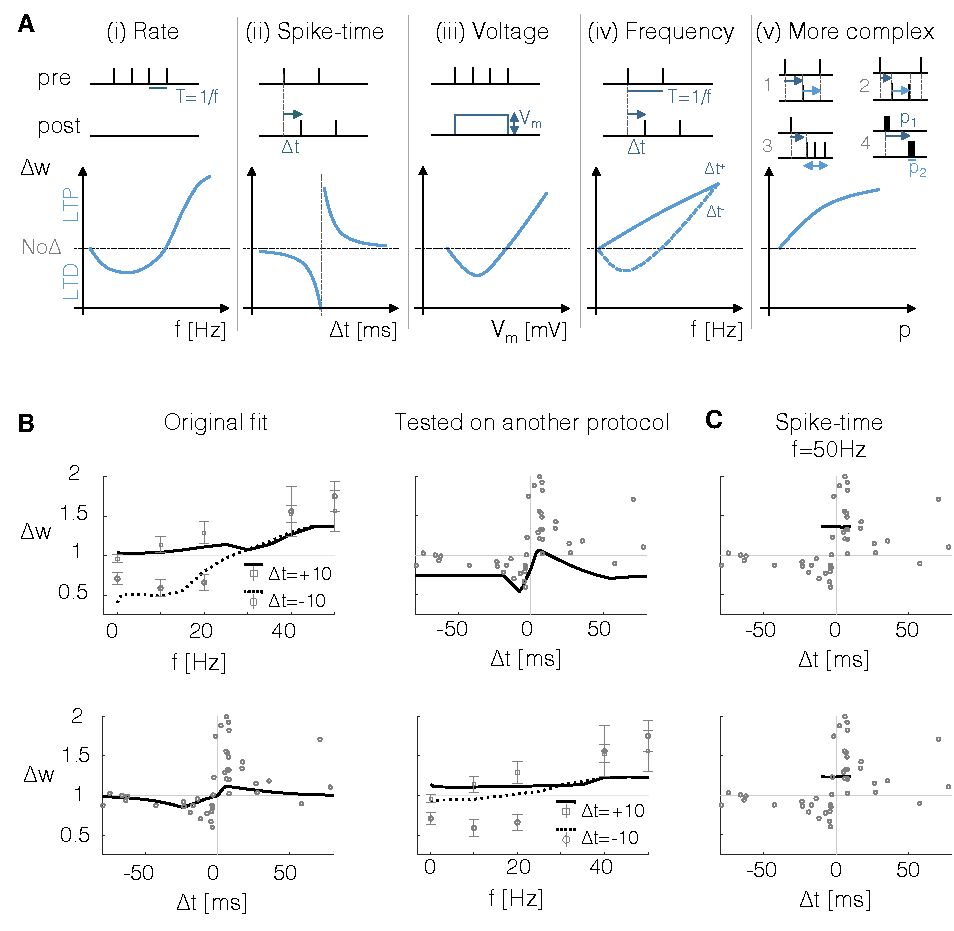
\includegraphics{fig/Review/Protocols.pdf}
    \caption{\textbf{Fitting of synaptic palsticity rules.} \textbf{A.} \textit{Experimental plasticity induction protocols are numerous.} (Top) The pre-post spiking activity is externally stimulated with a control parameter and a tested parameter. (Bottom) The evolution of the synaptic change ($\Delta w$) as function of the tested parameter. LTP and LTD refer to long-term potentiation and long-term depression. Rate protocol: the presynaptic neuron is spiking at a varying frequency $f$ \citep{dudek_homosynaptic_1992,bliss_long-lasting_1973}. (ii) Spike-time dependent plasticity: the presynaptic and postsynaptic neuron are both spiking at a given frequency (often 1Hz) with a changing delay $\Delta t$ between them \citep{bi_synaptic_1998} . (iii) Voltage: the presynaptic neuron is spiking and the postsynaptic is depolarized at a changing voltage membrane $V_m$ \citep{artola_different_1990, sjostrom_rate_2001}. (iv) Frequency-dependent induction protocol: both neurons are spiking at a frequency $f$. The presynaptic are preceding the postsynaptic spikes by $\Delta t^+=10$ms (or in the other way, post-pre $\Delta t^-=-10$ms \citep{sjostrom_rate_2001}. More complex protocols: others induction protocols using diverse tested parameters $p$. 1. Triplet: the time delay between the pre-post-pre is considered. 2. Quadruplet: the time delay between pre-post-post-pre. 3. Several postsynaptic spikes after a certain delay, the parameters are the number of spikes or the spiking frequency. 4. Bursting protocols: the burst duration and the burst delay are used to test the synaptic change. \textbf{B.} \textit{Synaptic rules fitted on one protocol cannot reproduce another protocol.} (top) The triplet model fitted on the frequency protocol (right) does not fit the spike-time protocol (left).  (bottom) The triplet model fitted on the spike-time protocol (right) does not fit the frequency protocol (left). Two parameter sets are required to fit the two different protocols. \textbf{C.} At 50Hz, whatever the parameter sets, the synaptic weight is potentiating. }
    \label{fig:ProtocolRecap}
\end{figure}


\subsection{To be (connected) or not to be}
Synaptic plasticity rules provide equations to describe one common goal: a definition for synaptic change. They are constrained by the same experimental \textit{in vitro}/in-vivo data. Since many years, theoreticians argue to show the relationships or the discrepancy between the different rules. 
 
For phenomenological models of plasticity, relationships are found in spite of their different implementations. Triplet model is an amelioration of the classical pair-based model to match a wider variety of experimental protocols \citep{pfister_triplets_2006}. It has been shown that it can also be mapped to rate-based learning rule as the BCM \citep{gjorgjieva_triplet_2011}. The sliding threshold of \citep{bienenstock_theory_1982} theory is also derived by introducing metaplasticity and other time-scales in the model \citep{el_boustani_stable_2012}.
Voltage-based model is actually an extension of triplet model \citep{clopath_connectivity_2010}. Heterosynaptic plasticity is reproduced by using a STDP rule combined with metaplasticity \citep{benuskova_stdp_2007}.

Similar mappings are shown in calcium-based rules. As mentioned in section XX, calcium-based rules are either described by a two-thresholds calcium function \citep{graupner_natural_2016} or a sigmoid calcium function \citep{shouval_converging_2002}. However, the two formulations are identical and they can be expressed by a generic model: $\tau([Ca]) \dot{w} = \Omega([Ca]) - w$ where $\tau([Ca])$ is the calcium-dependent time constant, $\Omega([Ca])$ is the calcium-dependent steady-state value. The coefficient identification is done in \citep{jacquerie_switches_2022}.

Then, phenomenological and biophysical models are often compared as shown in \citep{yeung_selectivity_2003, graupner_natural_2016, graupner_natural_2016, babadi_stability_2016}. 

\subsection{The apple does not fall far from the tree ?}
\textcolor{gray}{Je peux essayer de faire une sorte de petite arbre généalogique: Claudia Clopath a travaillé longtemps avec Wulfram Gerstner. Pfister est également un "enfant" de Gerstner. Rossum il a travaillé avec Gina turrigano (...) }


 
% ---------------------------------------------
% ---------------------------------------------
%
%       SMALL COMPUTATIONAL EXPERIMENTS 
%   TO SHOW INCOMPATIBILITY BETWEEN VAR & SP 
%
% ---------------------------------------------
% ---------------------------------------------
\section{Part IV - Incompatibility between synaptic plasticity rules, neuromodulation and biological variability}


% ---------------------------------------------
%                   experience 1
% ---------------------------------------------
\subsection{Synchronous bursting is not synchronous tonic}
Synaptic plasticity has been commonly studied in very stereotyped spiking protocol (see \textcolor{gray}{Figure Protocol}). For example, Spike-timing-dependent plasticity (STDP) relies on the exact spike timing between a presynaptic neuron and a postsynaptic neuron, driving either potentiation or depression \citep{bi_synaptic_1998}. Plasticity rules are fitted on such protocols and are able to reproduce synaptic changes acquired experimentally in spiking activity (see Figure \ref{fig:synchr}, tonic activity). However, neurons \textit{in vivo}  are not spiking as regularly as in these control conditions. Here we challenge the robustness of the plasticity rules during bursting activity where the emphasis is not focused on the spike-time itself but rather on the synchronicity of the whole rhythmic activity. To do so, we perform a simple computational experiment using a neuron circuit capable of switching between asynchronous spiking and rhythmic bursting states \citep{jacquerie_robust_2021, jacquerie_switches_2022}. Using a conductance-based modeling paradigm, the circuit reproduces the activities observed in cortical networks during switches in brain states \citep{mccormick_sleep_1997, zagha_neural_2014,chrol-cannon_computational_2014} among others. An inhibitory neuron projects GABA currents onto two excitatory neurons connected by an AMPA current (Figure \ref{fig:synchr}, right. See \nameref{sec: methods} for details). The synaptic strength between the two neurons is affected by synaptic plasticity, modeled either by a biophysical rule (two-threshold calcium levels established by \citep{graupner_natural_2016}) or a phenomenological rule (triplet rule from \citep{pfister_triplets_2006}). The circuit is able to switch from tonic to burst. This transition is driven by neuromodulators. These signaling substances are capable of changing the circuit state \citep{marder_neuromodulation_2014}. Neuromodulators are dynamically regulated, \textit{i.e.} their quantity is fluctuating across time. Even for one given brain state, variability in the concentration is observed. Here, we induced a small fluctuation of 5$\%$ during the burst rhythms. The endogenous burst remains similar with the qualitatively same intraburst frequency and duty cycle.  However, the evolution of the synatic weight computed by the two models lead to distinct behaviours. Indeed,  the phenomenological model is very sensitive to this small change in neuromodulator level, barely visible to the naked eyes (see Figure~\ref{fig:synchr}, bottom trace). The spike times are slightly shifted from mainly pre-post pattern inducing potentiation to post-pre pattern inducing depression (see zoom in Figure \ref{fig:synchr}) impacting drastically the time evolution of the weight. By contrast, biophysical models are blind to this perturbation. The calcium dynamic is driven by the burst itself and not the relative spike time inside the burst. The phenomenological rules are not adapted to capture plasticity in more complex firing activity \citep{gjorgjieva_burst-time-dependent_2009, jacquerie_switches_2022}.



\begin{figure}[H]
    \centering
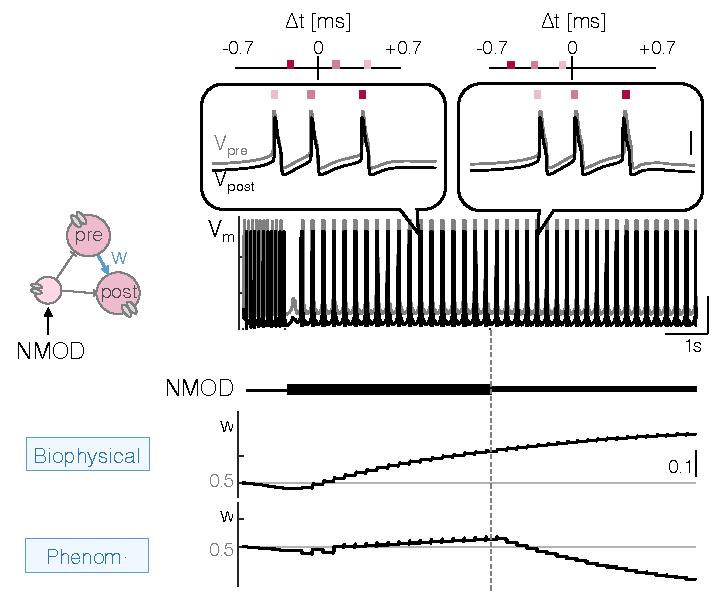
\includegraphics[scale=1]{fig/Review/fig_part3_synchr.pdf}
    \caption{\textbf{Phenomenological rules are sensitive to the relative spike times within an endogenous burst rhythm.} A 3-cell circuit composed of an inhibitory neuron connected to two excitatory neurons that have a plastic connection. Each neuron is a conductance-based model.
    Two seemingly similar patterns driven by slightly different neuromodulator levels (change in black bar size) lead to a slight difference on the pre-post pairing (pink squares on $\Delta t$). It results in an opposite synaptic weight change for phenomenological models (phenom.). On the contrary, biophysical model is blind to the change in neuromodulator level. (yscale-zoom: 50mV, time window-zoom: 90ms, voltage yscale: 50mV, , gray and black voltage traces are respectively the pre and postynaptic neuron activity).}
    \label{fig:synchr}
\end{figure}

% ---------------------------------------------
%                   experience 2
% ---------------------------------------------
\subsection{All synaptic plasticity rules are not suitable to handle intrinsic variability}
Neurons are highly variable in types, shapes, and even within the same category of neurons, intrinsic parameters are vastly different \citep{marder_multiple_2011}. Similar circuit activities can result from a large set of intrinsic conductances. These conductances are also ongoing turnover or they are under the control of neuromodulators. Here, we challenge the compatibility between synaptic plasticity rules and intrinsic variability. We use the same circuit in asynchronous spiking activity. Two intrinsic conductances are modified by 25$\%$ to 50$\%$. The activity is not perturbed but the evolution of the synaptic weight is different between the biophysical and the phenomenological rules (see Figure \ref{fig:intrinsic}). This difference in robustness comes from the driving mechanisms of the synaptic rule. For phenomenological models, the spike time is blind to change in intrinsic parameters. By contrast, the biophysical models are translating the calcium fluctuations into synaptic weight change. The intrinsic variability affects the calcium ion channels resulting in a change of intracellular calcium concentration, drastically impacting the evolution of the synaptic weight. It raises the controversy such tat two circuits with a similar activity but different sets of ion channels are supposed to have the same synaptic change (as seen in phenomenological rules) or these intrinsic differences drive different behavior in the synaptic connection. 


\begin{figure}[H]
    \centering
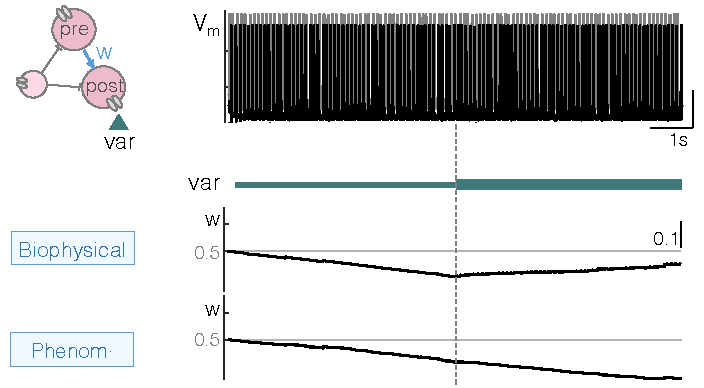
\includegraphics[scale=1]{fig/Review/fig_part3_intrinsic.pdf}
    \caption{\textbf{Change in intrinsic parameters affects the outcome of the biophysical models}. A 3-cell circuit composed of an inhibitory neuron projecting to two excitatory neurons whom synaptic strength is plastic. Each neuron is a conductance-based model. The circuit is in asynchronous spiking regime. As soon as the postsynaptic neuron conductance is affected by variability (var) mimicking the effect of neuromodulator, the outcome of the biophysical rule is affected. The phenomenological rule (Phenom.) is blind since the spiking activity is not modified. (Voltage scale: 50mV, gray and black voltage traces are respectively the pre and postynaptic neuron activity) }
    \label{fig:intrinsic}
\end{figure}

% ---------------------------------------------
% ---------------------------------------------
%
%               Conclusions Review
%
% ---------------------------------------------
% ---------------------------------------------
\subsection{Conclusion and perspectives}
\color{gray}
- J'aimerais bien orienter la conclusion en expliquant un peu comme eve marder que ce n'est pas forcément la moyenne des résultats de plasticité qui va donner une loi uniforme qui va fonctionner pour tous les modèles. 
Que c'est un peu comme reproduire une activité électrique d'un neurone, il y a pleins de combinaisons possibles de paramètres qui va fonctionner. Que ces règles sont aussi capabables de s'adapter via les neuromodulateurs pour respecter le fonctionnement du neurone. Mais le probleme dans la litérature actuelle c'est qu'on essaye de tuner les règles soit pour reproduire parfaitement des protocoles expérimentales qui sont très stéréotypés soit on construit des règles pour observer un phénomène d'apprentissage bien précis. - - - ca reste encore flou dans ma tête. 
- consider protocols with noise or more in vivo-like firing activity (example: \cite{cui_robustness_2018}).\\
- [Suvrathan, 2018] "In summary, coincidence-based rules for synaptic plasticity are no longer sufficient to explain the diversity of ways neural circuits can adapt and learn. The rules for plasticity can cover much longer timescales than previously thought and vary depending on the circuit they are embedded in, forcing both a reevaluation of the synaptic basis of learning rules as well as investigation into underlying mechanisms that can bridge long timescales"\\
- STDP in neural network (machine learning) >>  alors qu'on a montré que ce n'était pas robust 



\color{black}

\section{Methods}
\label{sec: methods}
Simulations were performed using the Julia programming language \cite{bezanson_julia_2017}. Data processing were performed either in Matlab. Code files are freely available at \url{https://github.com/KJacquerie/Review}.


\subsection{Neuron model and synaptic plasticity rules}
\label{sec: plasticity}
A 3-cell circuit was modeled using a conductance-based model. The neuronal model is the same used in \citep{jacquerie_switches_2022}. The inhibitory cell controls the rhythm of the circuit. An hyperpolarizing current applied to the inhibitory neuron switches the whole circuit in rhythmic bursting mode. This hyperpolarizing current models the effect of a neuromodulator signal (NMOD) \citep{zagha_neural_2014}. 

Regarding the plasticity between the pre- and postsynaptic cells, we used the triplet model defined in \citep{pfister_triplets_2006} for the phenomenological rule and the calcium-based model is defined in \citep{graupner_natural_2016}. More information is available \textcolor{gray}{SI Appendix or \citep{jacquerie_switches_2022}}.



\subsection{Computational experiments}

Figure \ref{fig:synchr} shows a neuronal switch from tonic to burst induced by neuromodulation with variable neuromodulator drive. Tonic activity is simulated by inducing spikes in the pre and postsynaptic cells with a strong current $I_{\mathrm{app}} = 50 \mathrm{nA}/\mathrm{cm^2}$ for a short duration of 3ms at a frequency of 10 $\mathrm{Hz}$ for 1s. The interspike intervals follow an independent Normal Distribution $\mathcal{N}(\frac{1}{f_0}, (\frac{\num{0.1}}{f_0})^{2})$, $f_0 = 10\mathrm{Hz}$. Then, A current $I_{\mathrm{app},\mathrm{I}} = -1.2 \mathrm{nA}/\mathrm{cm^2}$ is then applied to the inhibitory cell to mimic the impact of neuromodulators and induce bursting. After 6s, the applied current is changed to $I_{\mathrm{app},\mathrm{I}} = -1.\mathrm{nA}/\mathrm{cm^2}$. 

Plasticity is implemented between the pre- and postsynaptic neurons using the triplet and the calcium-based model mentioned above. The synaptic weight (w) evolution shows that both plasticity rules evolve the same in tonic mode according to the pairing protocol \citep{sjostrom_rate_2001}. However, the switch to burst induce divergent results between the two types of rules.\\

Figure \ref{fig:intrinsic} shows a tonic firing pattern with differences in the $g_{\mathrm{CaT}}$,  $g_{\mathrm{K,Ca}}$ conductances and affecting the postsynaptic calcium influx (more specially the parameter $C_{\mathrm{post}}$ in the calcium-based model \citep{graupner_natural_2016}). Spikes are generated by applying a strong current $I_{\mathrm{app}} = 50 \mathrm{nA}/\mathrm{cm^2}$ for a short duration of $3\mathrm{ms}$. The interspike intervals following independent Normal distributions $\mathcal{N}(\frac{1}{f_0}, (\frac{\num{0.1}}{f_0})^{2})$, $f_0 = 10\mathrm{Hz}$. From 0 to $5.5\mathrm{s}$, conductances values are  $g_{\mathrm{CaT}}=0.55$, $g_{\mathrm{K,Ca}}=4$, $C_{\mathrm{Post}}=1.62138$. Then, $g_{\mathrm{CaT}}=0.55\cdot1.5$, $g_{\mathrm{K,Ca}}=4\cdot0.75$, $C_{\mathrm{Post}}=1.62138\cdot 1.5$.
